\chapter{Wyniki sieci}
Wytrenowana sieć potrafi przejechać zarówno cały tor na symulatorze jak i
podziemny garaż instytutu. Na dodatek sieć trenowana pod symulator uczyła się,
tylko jeździć przeciwnie do ruchu wskazówek zegara, a po ustawieniu modelu w przeciwnym
kierunku potrafi przejechać cały tor bezproblemowo.

\section{Na co zwraca uwagę}
Aktywność sieci dla obrazków została wygenerowana za pomocą metody
Integrated Gradients\footnote{\href{https://arxiv.org/abs/1703.01365}{https://arxiv.org/abs/1703.01365}}.

Co było oczywiste w przypadku symulatora,sieć zwraca głównie uwagę na miejsca,
gdzie pojawiają się granice drogi\ref{sim_act}. Co ciekawe reaguje też na ścianę
tworzącą horyzont, ponieważ zmienia wygląd w zależności od odległości i może
pomóc w orientacji (na tej trasie).
\begin{figure}
  \centering
  \fbox{
  \scalebox{0.5}{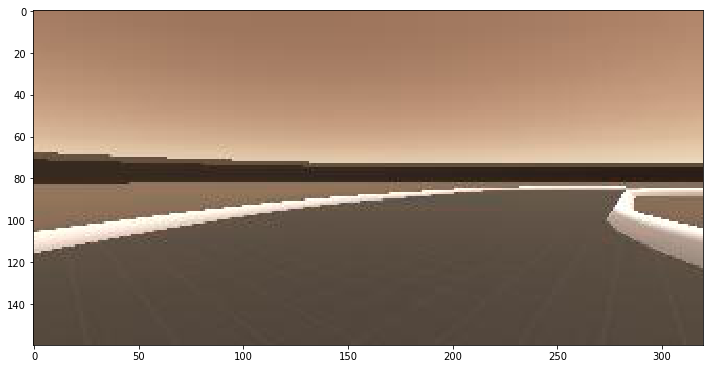
\includegraphics{img/sim_img.png}}
  }
  \label{sim_img}
  \caption{Obraz z symulatora}
\end{figure}
\begin{figure}
  \centering
  \fbox{
  \scalebox{0.5}{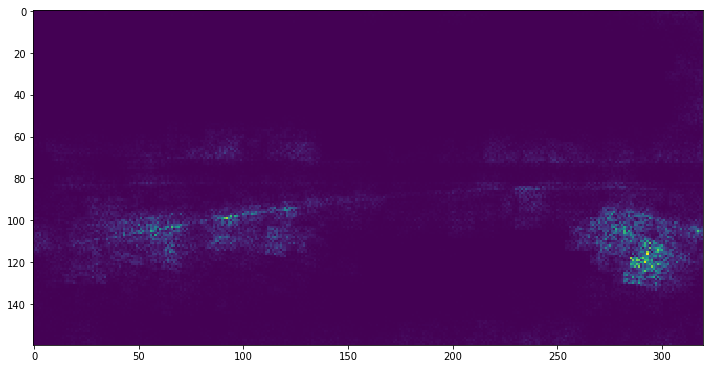
\includegraphics{img/sim_img_act.png}}
  }
  \label{sim_act}
  \caption{Na co sieć patrzy, symulator}
\end{figure}
\begin{figure}
  \centering
  \fbox{
  \scalebox{0.5}{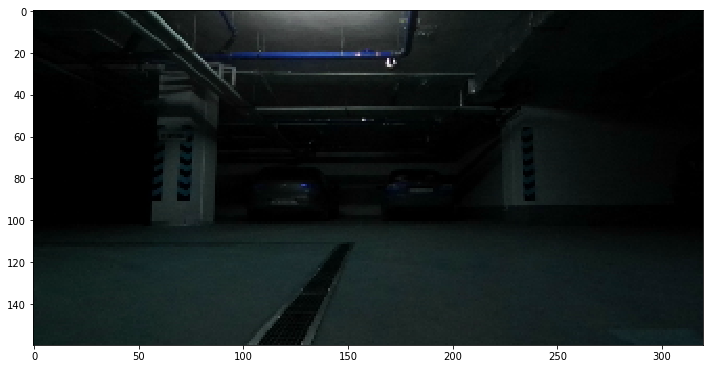
\includegraphics{img/real_img.png}}
  }
  \label{real_img}
  \caption{Obraz z nagrania}
\end{figure}
\begin{figure}
  \centering
  \fbox{
    \scalebox{0.5}{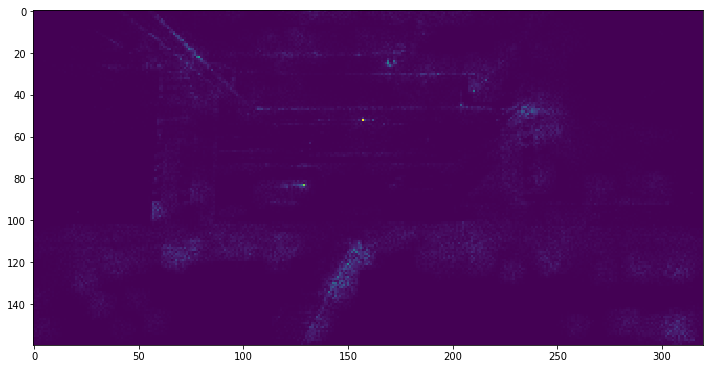
\includegraphics{img/real_img_act.png}}
  }
  \label{real_act}
  \caption{Na co sieć patrzy, nagranie}
\end{figure}

Z kolei dla łazika intensywność w najbardziej aktywnym miejscu jest dużo mniejsza,
co oznacza że nie sugeruje się tylko jednym miejscem. Ale mimo tego najbardziej 
zwraca uwagę na kratkę na podłodze, która mogła by wystarczyć do nawigacji.

\section{W porównaniu do nagrania}
Na wykresie \ref{plot_ang} widać że sieć (pomarańczowy kolor), mniej gwałtownie 
zmienia szybkość obrotu niż kierowca (kolor niebieski). Ale w podobnych momentach
zauważa, że należy skręcić.
\begin{figure}
  \centering
  \fbox{
    \scalebox{0.5}{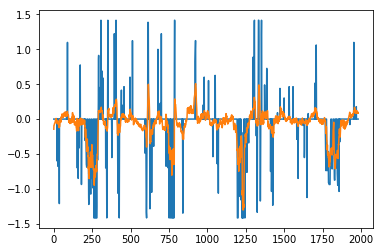
\includegraphics{img/real_data_ang.png}}
  }
  \label{plot_ang}
  \caption{Prędkość obrotowa: sieć vs kierowca}
\end{figure}

\section{Wpływ architektury}
W przypadku sieci pod symulator, usunięcie niektórych warstw konwolucyjnych
pozwalało modelowi utrzymać się na torze, a taka sama zredukowana architektura 
nie radziła sobie dobrze w przypadku nagrań z prawdziwego łazika. Natomiast
usunięcie nieliniowości z warstw konwolucyjnych tak okaleczyła zdolności sieci,
że nie potrafiła się utrzymać na wirtualnym torze.

Z kolei usunięcie dropoutu, bardzo szybko powodowało overfitting i radziła sobie
dobrze tylko na danych uczących. Z kolei dodanie warstw liniowych na końcu nie 
poprawiało, ani nie pogorszało zbytnio wydajności sieci, przynajmniej dla
nagrań z symulatora. Widocznie większość interesujących cech już jest znaleziona
w ramach konwolucji, i dla tak prostych danych nie pomaga zwiększenie modelu.

Co ciekawe w przypadku wytrenowanego już modelu do symulatora zredukowanie 
rozdzielczości obrazów dziesięciokrotnie w każdym wymiarze(z rozdzielczości 
320x160 do 32x16),
i zwykłe przeskalowanie w górę przed zewaluowaniem wystarczy żeby urzymać się 
na torze.

Na dodatek sieć uczona na obrazie kolorowym bezproblemowo działa, gdy
zredukuje się obraz do skali szarości a następnie powtórzy kanał trzykrotnie.

